% !TeX spellcheck = de_DE
\section{Simulation mit Netgen und Matlab}

Alle Unterlagen f�r den 3ten �bungsteil finden Sie im TUWEL-Kurs. Installieren Sie Netgen 6.1. Das Simulationsbeispiel finden Sie in Simulations.zip im Verzeichnis Electrostatics.
Falls Sie nach ernsthaften Anstrengungen immer noch ein Problem mit der Installation oder den Simulationen haben, dann schreiben Sie einfach ein Email an karl.hollaus@tuwien.ac.at und schildern kurz das Problem.
\\
\\

{\large Angabe}
\begin{enumerate}
	\item Plattenkondensator(Verwenden Sie das Problem Electrostaics\_2Domains.pde)
	\begin{enumerate}
		

	\item Bestimmen Sie die Kapazit�t des Plattenkondensators mit Hilfe einer FE-Simulation und vergleichen Sie diese mit der bekannten N�herungsformel. Die Plattenbreite ist $b = 6m$, der Plattenabstand ist $d = 2m$ und die Spannung an den beiden Platten betr�gt $U=2V$.
	\item Untersuchen Sie den relativen Fehler in Abh�ngigkeit vom Dielektrikum zwischen den Kondensatorplatten. Stellen Sie den relativen Fehler in Abh�ngigkeit von $\epsilon_r$ dar.
	\item Untersuchen Sie den Einfluss des fernen Randes auf die L�sung indem Sie die Geometrie des Problemgebietes vergr��ern bzw. verkleinern. Dokumentieren Sie Ihre Erkenntnisse.
		\end{enumerate}
\end{enumerate}

\subsection{Plattenkondensator Simulation}
\begin{figure}[h]
	\centering
	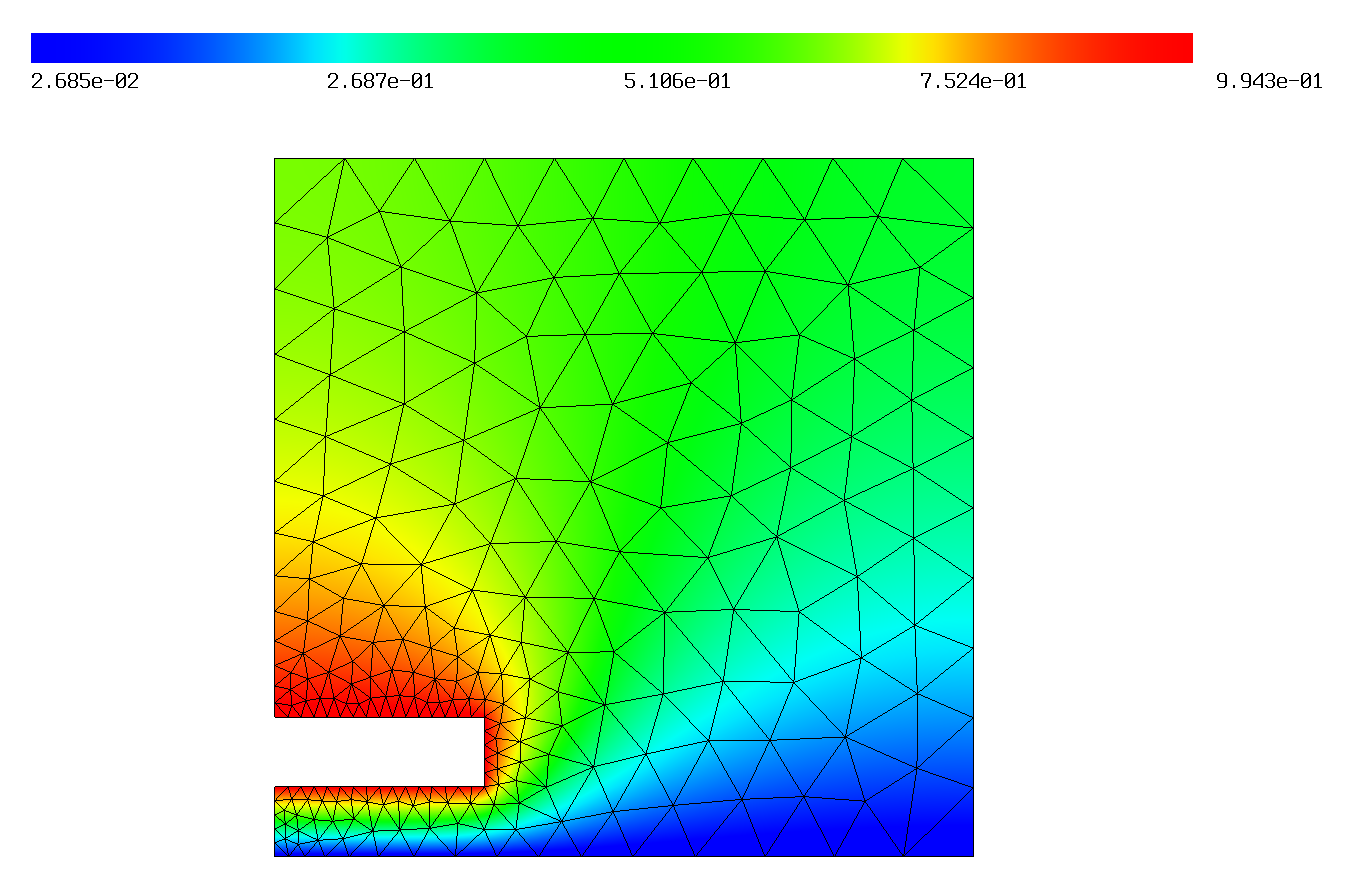
\includegraphics[width=0.7\linewidth]{../Netgen/pde1}
	\caption{Simulation eines Plattenkondesators mit Netgen}
	\label{fig:pde1}
\end{figure}

\subsection{Einfluss des fernen Randes}

Die Gr��e des berechneten Gebiets, und damit die "N�he" der Randbedingungen zueinander haben einen gro�en Einfluss auf das sich um den Kondensator ergebende Streufeld. Es wurde aus Symmetrie-Gr�nden nur der linke, obere Teil eines Kondensators in 2D berechnet.
F�r die Berechnung in Matlab wurden folgende Werte verwendet: 
\begin{itemize}
	\item $1m = 0.1 \text{Skaleneinheiten}$
	\item PDGL: $ - \nabla \cdot c \nabla u = 0$ wobei $c=1$ ist.
	\item Dirichletsche Randbedingungen an den Kondenstorfl�chen, an der horizontalen Symmetrie-Achse, sowie am fernen Rand (rechts und oben).
	\item Neumansche Randbedingung an der vertikalen Symmetrie-Achse
\end{itemize}
\textit{Info:} Aufgrund anhaltender Installatiosprobleme mit Python unter OS X wurden alle Simulationen mit dem \textit{pdetool} von Matlab gemacht. 

\begin{figure}[ht]
	\centering
\begin{tabular}{cc}
\begin{subfigure}{0.45\textwidth}
	\centering
	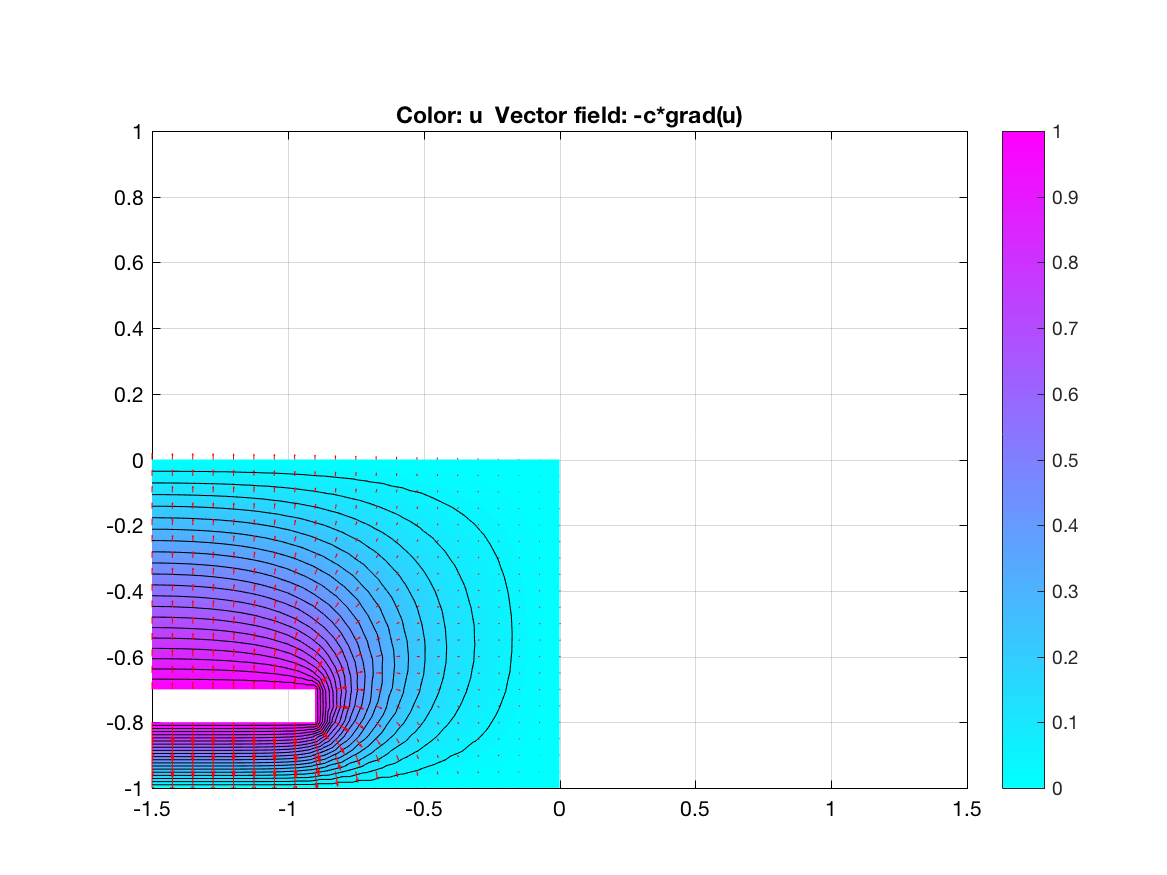
\includegraphics[width=\linewidth]{../Netgen/pdetool/pde-near}
	\caption{Rand sehr nah, 1.5 x 1}
	\label{fig:pde-near}
\end{subfigure} &
\begin{subfigure}{0.45\textwidth}
	\centering
	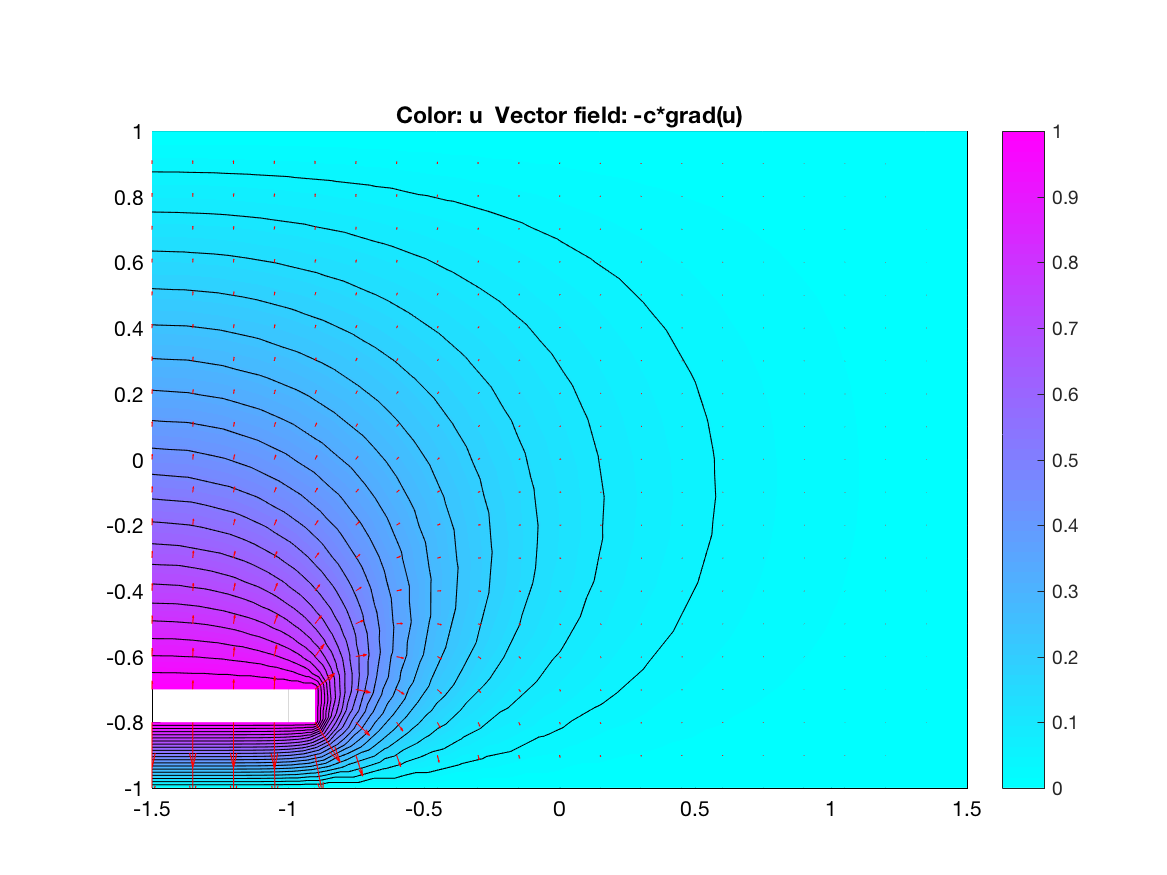
\includegraphics[width=\linewidth]{../Netgen/pdetool/pde-far}
	\caption{Rand nah, 3 x 2}
	\label{fig:pde-far}
\end{subfigure} \\
\begin{subfigure}{0.45\textwidth}
	\centering
	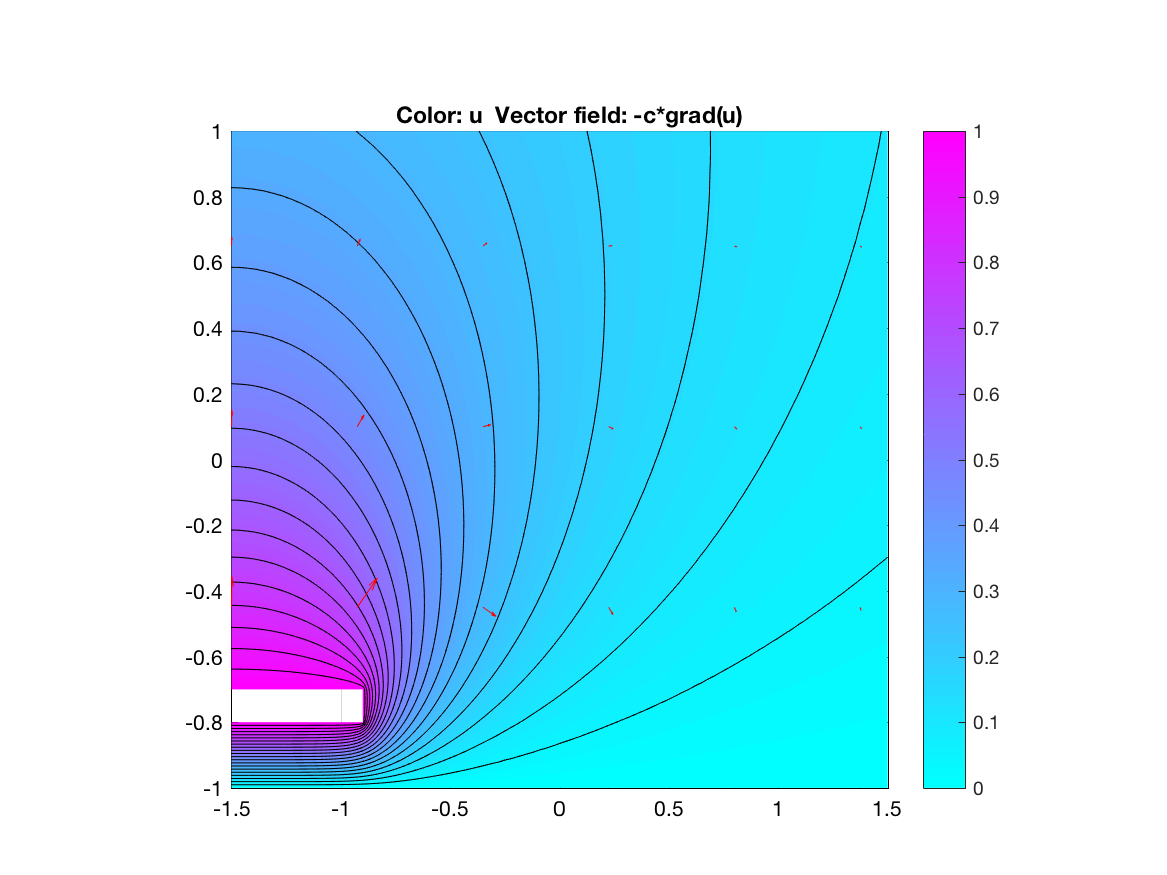
\includegraphics[width=\linewidth]{../Netgen/pdetool/pde-not-so-very-far}
	\caption{Gro�es Gebiet 10 x 10}
	\label{fig:pde-far}
\end{subfigure} &
\begin{subfigure}{0.45\textwidth}
	\centering
	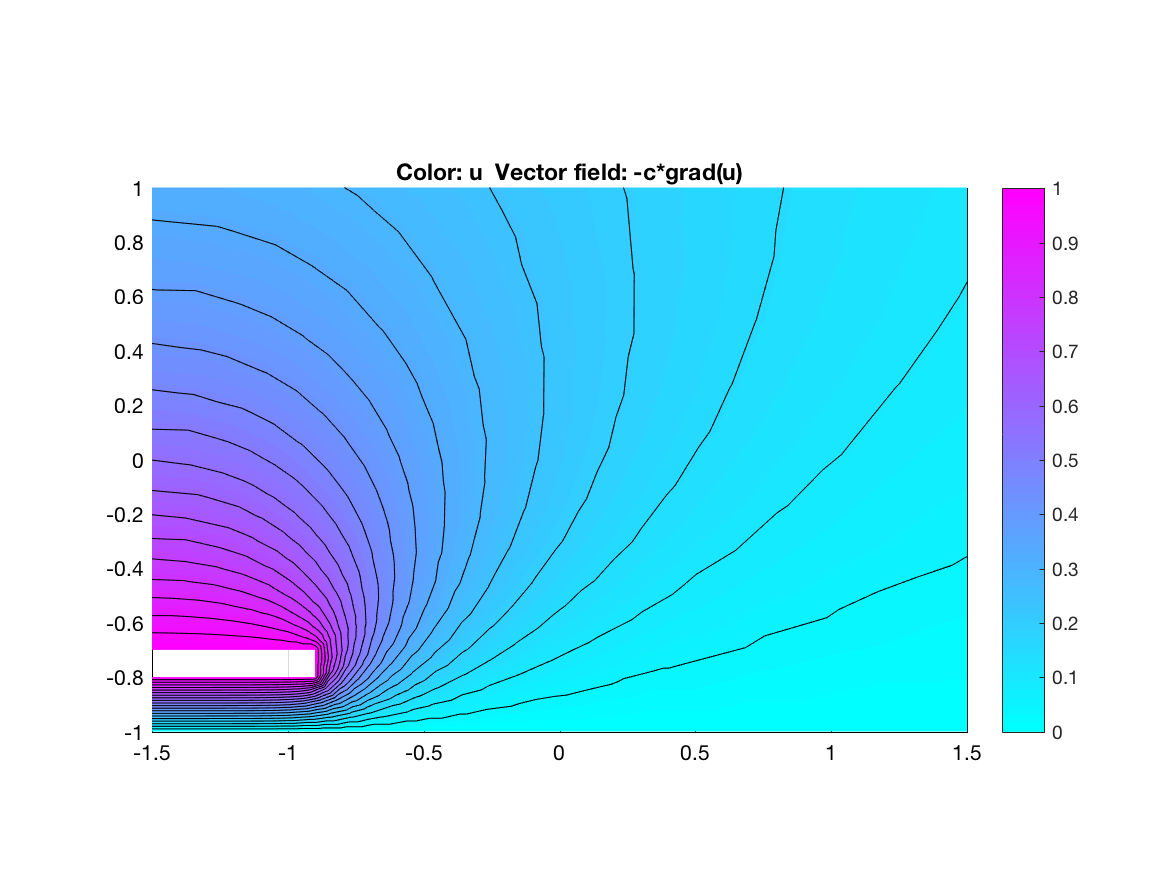
\includegraphics[width=\linewidth]{../Netgen/pdetool/pde-very-far}
	\caption{Riesen Gebiet 100 x 100}
	\label{fig:pde-far}
\end{subfigure}
\end{tabular}
\caption{Untersuchen des Einflusses des fernen Randes}
\end{figure}